\section{Results}
\label{sec:results}

\subsection{Q1: How much memory does quantization actually save?}
\label{sec:q1}

\begin{figure}[t]
\centering
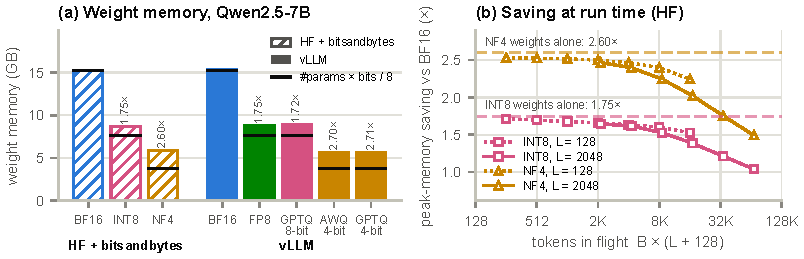
\includegraphics[width=\linewidth]{q1_memory_main}
\caption{\textbf{Q1: the real saving is smaller than the bit-width suggests.} (a)~Weight memory of
Qwen2.5-7B measured after loading (bars) against the naive estimate $\#\text{params}\times\text{bits}/8$
(black ticks); labels give the saving against BF16 on the same backend. (b)~Saving of the peak
memory on HF as more tokens are in flight (dashed: the saving of the weights alone).}
\label{fig:memory}
\end{figure}

\answer{Less than the bit-width suggests, and less as the context grows. On vLLM, the saved memory
becomes room for more requests.}

\textbf{Weights.} The naive estimate is too low for every format, by up to \NaiveExcessMax\% for NF4
(\cref{fig:memory}a). Only the decoder's linear layers are quantized: the embedding and the LM head
(\EmbedShareSeven\% of Qwen2.5-7B's parameters) stay in 16 bits, and each format stores scales.
Counting these parts predicts every HF measurement within \ModelErrMax\% (\cref{app:memory}). So
4-bit weights shrink the 7B model by \WtNFSeven{} (NF4) to \WtAWQSeven{} (AWQ-INT4), and 8-bit weights
by \WtIntEightSeven.

\textbf{Run time.} The KV cache and the activations are not quantized, so the saving shrinks as more
tokens are in flight (\cref{fig:memory}b). NF4 cuts the peak memory of one short request by
\MemSmallNF, but that of 32 requests of 2048 tokens by only \MemBigNF; LLM.int8(), which keeps extra
copies of the activations, by \MemBigInt. On HF, the 7B model runs out of memory at $B=64$, $L=2048$ in
every format, because the prefill activations fill the GPU.

\textbf{Capacity.} vLLM turns all the memory the weights leave free (within 85\% of the GPU) into KV
cache. With AWQ-INT4, Qwen2.5-7B holds \KVratioAWQ{} as many cached tokens as with BF16 (\KVawqSeven{}
vs.\ \KVbfSeven). \FourteenNote{}

\subsection{Q2: How do latency and throughput change?}
\label{sec:q2}

\begin{figure}[t]
\centering
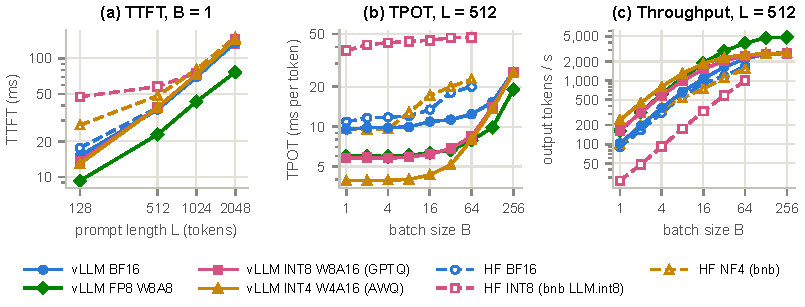
\includegraphics[width=\linewidth]{q2_latency_throughput}
\caption{\textbf{Q2: latency and throughput of Qwen2.5-7B} with 128 generated tokens. (a)~TTFT of one
request; (b)~TPOT and (c)~output throughput for 512-token prompts. Solid lines: vLLM; dashed lines
with hollow markers: HF with bitsandbytes.}
\label{fig:latency}
\end{figure}

\answer{With fused kernels, fewer bytes give an almost proportional decode speedup for small
batches; with bitsandbytes they do not. No weight-only format shortens prefill.}

\textbf{Decode.} At batch size 1 (prediction P1), vLLM's BF16 step takes \TPOTbfVllmSeven\,ms,
within \BWutilVllm\% of the time needed to read the 15.2\,GB of weights, so it is purely memory-bound.
On vLLM, fewer bytes do mean less time (\cref{fig:latency}b): AWQ-INT4 decodes \AWQspeedup{} faster
than BF16, GPTQ-INT8 \GPTQeightspeedup{} and FP8 \FPeightspeedup, which is \IdealAWQ--\IdealGQE\% of
their byte savings. On HF the same idea fails: LLM.int8() is \INTeightslowdown{} slower than BF16, and
NF4 is \NFsevenB{} faster on 7B (\NFfourteenB{} on 14B) but \NFthreeslow{} slower on 3B.
These are whole stacks: LLM.int8() and GPTQ-INT8 differ in method, activation path and engine, not
only in kernel. \Cref{sec:mechanism} separates the kernels from the rest.

\textbf{Prefill.} As P3 predicts, AWQ and GPTQ change the TTFT by at most \TTFTwoMax\%, and NF4 makes
it \TTFTnfSlow{} slower, because bitsandbytes dequantizes every weight matrix first
(\cref{fig:latency}a). FP8, which also quantizes the activations, makes a 2048-token prefill
\TTFTfpLong{} faster.

\textbf{Throughput.} At $B=256$ (\cref{fig:latency}c), AWQ-INT4 (\ThrAWQmax{} tokens/s) no longer
beats BF16 (\ThrBFmax), while FP8 reaches \ThrFPmax{} tokens/s, \ThrFPratio{} the BF16 rate. Energy
per token follows latency (\cref{app:speed}).

\subsection{Q3: When does lower precision pay off?}
\label{sec:q3}

\begin{figure}[t]
\centering
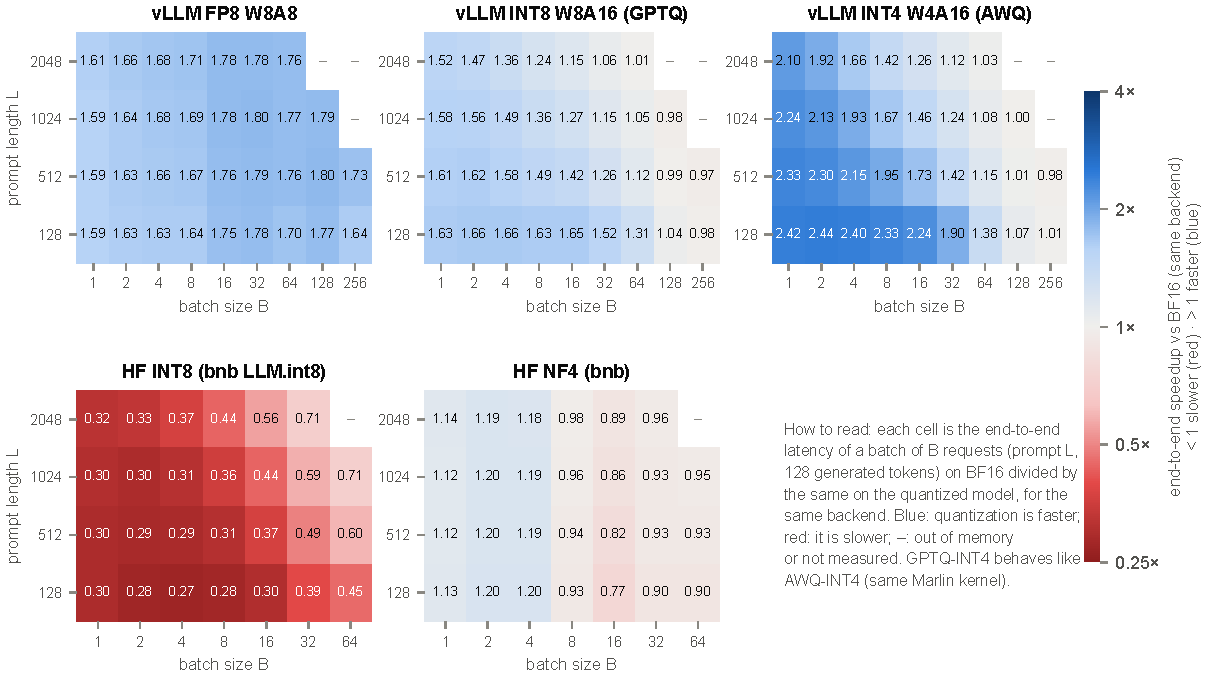
\includegraphics[width=\linewidth]{q3_speedup_heatmaps}
\caption{\textbf{Q3: where each format pays off.} End-to-end speedup of $B$ requests ($L$-token prompts,
128 generated tokens) over BF16 on the same backend, Qwen2.5-7B. Dashes: out of memory or not run.
GPTQ-INT4 behaves like AWQ-INT4 (\cref{tab:crossover} in \cref{app:speed}).}
\label{fig:heatmaps}
\end{figure}

\answer{Weight-only formats pay off for small batches, and their gain ends near the batch size at
which decoding becomes compute-bound. FP8 pays off everywhere; the bitsandbytes formats rarely do.}

\Cref{fig:heatmaps} maps the end-to-end speedup over batch size and prompt length. Three regimes
appear. (i)~\emph{Weight-only formats with fused kernels} (AWQ, GPTQ) win by up to \AWQmaxEtoE{} when
decode dominates. Their gain shrinks as the batch and the prompts grow, and AWQ-INT4 stops winning at
$B\approx\AWQcross$ for 512-token prompts, close to $M\approx R\approx\RidgeBF$, where BF16 decoding
itself becomes compute-bound (P2).
(ii)~\emph{FP8 W8A8} wins in every cell (\FPminEtoE--\FPmaxEtoE), because it halves the bytes
\emph{and} raises the compute roof. (iii)~\emph{bitsandbytes formats} rarely win: LLM.int8() is slower
in every cell (\INTminEtoE--\INTmaxEtoE), and NF4 wins only for 7B below $B\approx\NFcross$. Longer
answers raise the share of decode and push the crossover up: at $B=16$, AWQ-INT4 speeds up a request
with 32 output tokens by \OutAWQSixteenShort, but one with 512 output tokens by \OutAWQSixteenLong{}
(\cref{app:speed}).

\subsection{Why: kernels, the roofline and host overhead}
\label{sec:mechanism}

\begin{figure}[t]
\centering
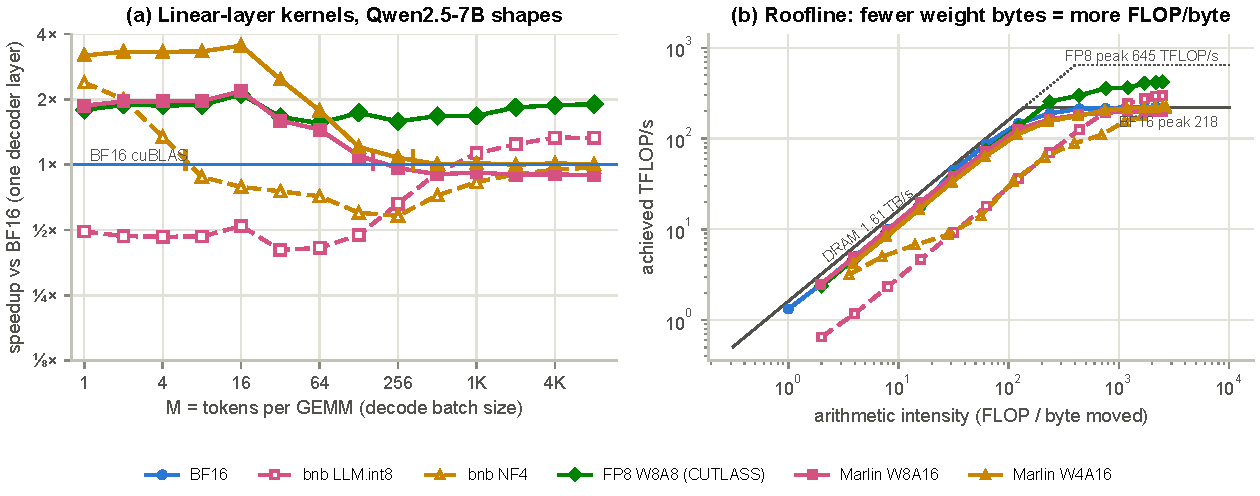
\includegraphics[width=\linewidth]{q3_kernel_crossover}
\caption{\textbf{Why the crossover happens.} (a)~Speedup of each low-bit kernel over BF16 cuBLAS on the
matrix shapes of one Qwen2.5-7B decoder layer, against the tokens $M$ per multiply (the decode batch
size); ticks mark where it falls below 1.05. (b)~The same kernels on the measured roofline.}
\label{fig:kernels}
\end{figure}

\answer{The roofline explains vLLM, where the kernels are fast. The CPU cost of launching kernels
explains HF, where the GPU is often idle.}

\textbf{Kernels.} We time each low-bit kernel alone on the matrix shapes of one 7B decoder layer
(\cref{fig:kernels}a). Marlin W4A16 is \MarlinFourMone{} faster than BF16 at $M=1$ and keeps a gain
above 5\% up to $M\approx\MarlinFourCross$; Marlin W8A16 starts at \MarlinEightMone{} and ends at
$M\approx\MarlinEightCross$. \Cref{fig:kernels}b shows why (P2): fewer bytes per weight move a kernel
up the bandwidth roof faster, but it hits the same BF16 compute roof. Real kernels approach the roof
gradually, so the crossovers lie somewhat above the ridge point. FP8 W8A8 is \FPkernMone{} faster at
$M=1$ and still \FPkernMmax{} at $M=8192$, because its compute roof is about three times higher
(\FPeightmeas{} vs.\ \BFmeas\,TFLOP/s). The bitsandbytes kernels are not slow everywhere: NF4's
kernel is \NFkernMone{} faster than BF16 at $M=1$ (it dequantizes whole matrices for larger $M$), yet
the whole NF4 model is only \NFsevenB{} faster. Time must be lost outside the kernels.

\begin{figure}[t]
\centering
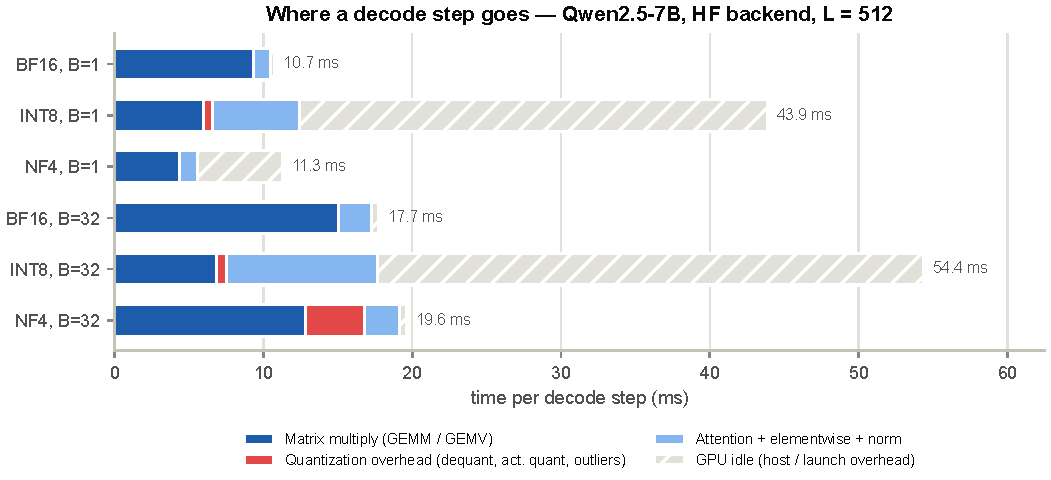
\includegraphics[width=\linewidth]{mech_decode_breakdown}
\caption{\textbf{Where an HF decode step goes} (Qwen2.5-7B, 512-token prompts): GPU time by kernel
type, and the time the GPU waits for the CPU (hatched).}
\label{fig:profile}
\end{figure}

\textbf{Host overhead.} \Cref{fig:profile} profiles one HF decode step of the 7B model. With BF16, the
GPU is busy \BusyBFone\% of the step. LLM.int8() launches \KernIntRatio{} as many kernels (casts,
outlier handling, quantization, two matrix multiplies per layer), and the GPU is busy only
\BusyIntone\% of the time: Python and kernel launches set the speed. NF4 lies in between (\BusyNFone\%
busy). More layers mean more launches, so the 36-layer 3B model suffers more than the 28-layer 7B
model. vLLM avoids most of this cost with CUDA graphs, which replay a decode step with very few launches.

\subsection{Do the results hold for real traffic?}
\label{sec:real}
\answer{Yes, and the serving system matters even more than the number format.}
In a replay of 300 ShareGPT requests (\cref{tab:serving_main} in \cref{app:real}), AWQ-INT4 gives the lowest TPOT with
one client (\SrvTPOTawqOne\,ms vs.\ \SrvTPOTbfOne\,ms for BF16), and FP8 the highest throughput with 64
clients (\SrvThrFP{} vs.\ \SrvThrBF{} tokens/s), as the crossover of \cref{sec:q3} predicts. With the
same 16 requests in flight, vLLM BF16 delivers \SrvGap{} the throughput of HF BF16. Both run BF16, so
this gap belongs to the serving stack (continuous~\cite{yu2022orca} vs.\ static batching, CUDA
graphs), not to quantization; the two stacks are also timed differently (\cref{app:real}).



\subsection{Q4: How much quality does quantization cost?}
\label{sec:q4}
\Cref{tab:quality,fig:quality} report WikiText-2 perplexity and GSM8K accuracy. Every GSM8K
comparison is paired: all configurations answer the same 1,319 questions, so we test each
difference against HF BF16 with an exact McNemar test on the questions where exactly one of the two
runs is correct.

\textbf{Noise floor.} Even two BF16 runs of the same weights disagree. vLLM and HF use different
kernels and accumulation orders, and greedy decoding turns the resulting rounding differences into
different reasoning chains: the two backends disagree on \BackendFlipsSeven{} of the 7B model's
questions and their accuracies differ by \BackendNoiseSeven{} points (\BackendNoiseThree{} for 3B).
Differences of this size are not caused by quantization.

\textbf{8-bit formats preserve quality.} LLM.int8(), GPTQ-INT8 and FP8 W8A8 stay within
\DEightAbsSeven{} GSM8K points and \PPLEightAbsSeven{} perplexity of BF16 on the 7B model
(\DEightAbsThree{} points on 3B), and \EightSentence.

\textbf{4-bit formats cost little on 7B and more on 3B.} The 4-bit formats raise perplexity by
\PPLFourMinSeven{} to \PPLFourMaxSeven{} on the 7B model, and its GSM8K accuracy changes by only
\DFourMinSeven{} to \DFourMaxSeven{} points, none significant. The 3B model loses
\DFourMinThree{} to \DFourMaxThree{} points with \PPLFourMinThree{} to \PPLFourMaxThree{}
perplexity, and \FourThreeSurvive{} of these drops remain significant after a Bonferroni correction:
a smaller model has less redundancy to absorb the rounding error.

\textbf{Model size versus bit-width.} \Cref{fig:quality} places every configuration by its weight
memory. \QualityGuide{} At a fixed memory budget, parameters are worth more than bits.

\textbf{One metric is not enough.} The 14B GPTQ-INT4 checkpoint scores \AccGPTQFourFourteenPct\%
on GSM8K, on par with the other 14B formats, yet its WikiText-2 perplexity is
\PPLGPTQFourFourteen{} against \PPLOthersFourteen{} for AWQ-INT4, GPTQ-INT8 and FP8. The outlier
is not an artifact of our setup: it persists with BF16 instead of FP16 activations, the loss is
elevated at every position of the 2048-token window, and the same harness scores the 7B GPTQ-INT4
checkpoint normally. Ranking the next token shows what happened. On raw WikiText the checkpoint predicts the
next token correctly only \TopOneGPTQWiki\% of the time (\TopOneOthersWiki\% for the other 14B
formats), whereas on chat-formatted GSM8K solutions it matches them (\TopOneGPTQChat\% vs.\
\TopOneOthersChat\%). The quantized weights still model the chat distribution they serve but have
lost much of their general language modeling. GSM8K alone would have missed this; perplexity alone
would have rejected a checkpoint that works for chat.

\begin{table}[t]
\centering
\footnotesize
\caption{Q4 --- quality. WikiText-2 perplexity (2048-token windows) and GSM8K accuracy (1,319 questions, zero-shot CoT, greedy decoding). Deltas are against HF BF16 of the same model; $p$ is the two-sided exact McNemar test of the paired GSM8K answers against HF BF16.}
\label{tab:quality}
\setlength{\tabcolsep}{3.2pt}
\begin{tabular}{llrrrrr}
\toprule
Model & Config & PPL & $\Delta$PPL & GSM8K (\%) & $\Delta$acc & $p$ \\
\midrule
3B & HF BF16 & 8.56 & -- & 85.8 & -- & -- \\
 & HF INT8 & 8.66 & $+0.10$ & 85.5 & $-0.3$ & 0.777 \\
 & HF NF4 & 9.11 & $+0.55$ & 82.6 & $-3.3$ & $<$0.001 \\
 & vLLM BF16 & 8.56 & $+0.00$ & 86.0 & $+0.2$ & 0.871 \\
 & vLLM FP8 & 8.64 & $+0.09$ & 85.4 & $-0.5$ & 0.610 \\
 & vLLM GPTQ-8 & 8.56 & $+0.00$ & 86.4 & $+0.6$ & 0.322 \\
 & vLLM AWQ-4 & 9.10 & $+0.54$ & 82.7 & $-3.1$ & 0.002 \\
 & vLLM GPTQ-4 & 9.22 & $+0.66$ & 82.0 & $-3.8$ & $<$0.001 \\
7B & HF BF16 & 7.46 & -- & 90.8 & -- & -- \\
 & HF INT8 & 7.49 & $+0.03$ & -- & -- & -- \\
 & HF NF4 & 7.77 & $+0.31$ & 90.3 & $-0.5$ & 0.500 \\
 & vLLM BF16 & 7.46 & $+0.00$ & 91.2 & $+0.4$ & 0.359 \\
 & vLLM FP8 & 7.51 & $+0.05$ & 90.8 & $+0.0$ & 1.000 \\
 & vLLM GPTQ-8 & 7.46 & $+0.00$ & 91.7 & $+0.9$ & 0.043 \\
 & vLLM AWQ-4 & 7.85 & $+0.39$ & 90.4 & $-0.5$ & 0.576 \\
 & vLLM GPTQ-4 & 7.78 & $+0.32$ & 91.1 & $+0.2$ & 0.828 \\
14B & vLLM FP8 & 5.77 & -- & 94.4 & -- & -- \\
 & vLLM GPTQ-8 & 5.71 & -- & 94.7 & -- & -- \\
 & vLLM AWQ-4 & 6.16 & -- & 93.9 & -- & -- \\
 & vLLM GPTQ-4 & 37.46$^{\ddagger}$ & -- & 93.7 & -- & -- \\
\bottomrule
\end{tabular}
\par\vspace{2pt}\parbox{\linewidth}{\scriptsize $^{\ddagger}$Degraded on raw text but not on chat-formatted text; see \cref{sec:q4}.}
\end{table}



\subsection{Do the results generalize? Qwen3-8B and Qwen3-32B}
\label{sec:general}
To check that the conclusions are not specific to Qwen2.5, we repeated the core measurements on
Qwen3-8B~\cite{qwen3}, a newer model with a different layout (\FamRLayers{} layers and \FamRKVheads{}
KV heads against \FamQLayers{} and \FamQKVheads{} for Qwen2.5-7B), run in non-thinking mode.
\Cref{tab:general} compares the two on the same grid.

The systems results carry over almost unchanged. 4-bit weights shrink by \FamRAWQsave{} rather than
$4\times$; at batch size one AWQ-INT4 decodes \FamRAWQone{} faster (\FamQAWQone{} for Qwen2.5-7B),
FP8 \FamRFPone{} faster, and LLM.int8() runs at \FamRINTone{} of the BF16 speed. At $B=\FamRBcmp$
FP8 still raises throughput by \FamRFPthr{} while AWQ-INT4 has fallen to \FamRAWQthr. The one
difference confirms the host-overhead explanation of \cref{sec:mechanism}: NF4, \FamQNFone{} faster
than BF16 on the 28-layer Qwen2.5-7B, is \FamRNFone{} on the 36-layer Qwen3-8B, just as it was
slower on the 36-layer Qwen2.5-3B. More layers mean more kernel launches per decode step, and the
step becomes bound by the host rather than by memory. Qwen3-8B also stores \FamKVratio{} as many
KV-cache bytes per token, so at $B=256$ none of its configurations fits the cache; the memory a
format saves on weights matters even more for such models. \FamQualitySentence

\textbf{Scaling up: Qwen3-32B.} At 32B parameters the question changes from speed to feasibility.
Qwen3-32B needs \BigBFw\,GB in BF16 and about half of that in FP8 or INT8, more than the GPU's
32\,GB, so on this GPU it runs only at 4 bits: AWQ-INT4 takes \BigAWQw\,GB and leaves room for
\BigAWQkv{} cached tokens, and NF4 takes \BigNFw\,GB. Against Qwen3-8B in BF16 (\SmallBFw\,GB, a
similar budget), the 4-bit 32B model needs \BigAWQtpot\,ms per decoded token at batch size one
(vLLM; 8B BF16: \SmallBFtpot\,ms) and scores \BigGSMawq\% vs.\ \SmallGSMbf\% on GSM8K
(\BigGAWQp) and \BigMMLUawq\% vs.\ \SmallMMLUbf\% on MMLU (\BigMAWQp). \BigVerdict{} One caveat is
numerical: the AWQ checkpoint ships FP16 activations, and in \BigNaNwin{} perplexity windows the
activations overflow beyond the first 512 positions and the loss becomes NaN; with BF16
activations every window is finite (perplexity \BigPPLawq), so long-context use of this
checkpoint should run in BF16.

\begin{table}[htbp]
\centering
\small
\caption{The main results for Qwen2.5-7B and Qwen3-8B (non-thinking mode) on the same grid (512-token prompts, 128 output tokens). Throughput is compared at the largest batch at which both models' KV caches hold every request ($B=64$). Qwen3-8B has no official GPTQ checkpoint.}
\label{tab:general}
\setlength{\tabcolsep}{3.2pt}
\begin{tabular}{lrr}
\toprule
Metric (vs.\ BF16) & Qwen2.5-7B & Qwen3-8B \\
\midrule
Weight saving, AWQ-INT4 (vLLM) & 2.70$\times$ & 2.67$\times$ \\
Weight saving, NF4 (HF) & 2.60$\times$ & 2.55$\times$ \\
Decode speedup $B=1$, AWQ-INT4 & 2.44$\times$ & 2.33$\times$ \\
Decode speedup $B=1$, FP8 & 1.59$\times$ & 1.54$\times$ \\
Decode speedup $B=1$, NF4 & 1.13$\times$ & 0.90$\times$ \\
Decode speedup $B=1$, LLM.int8() & 0.29$\times$ & 0.28$\times$ \\
Throughput $B=64$, AWQ-INT4 & 1.15$\times$ & 1.12$\times$ \\
Throughput $B=64$, FP8 & 1.76$\times$ & 1.67$\times$ \\
GSM8K $\Delta$ pp ($p$), FP8 & $0.0$ (1.000) & $+0.5$ (0.488) \\
GSM8K $\Delta$ pp ($p$), LLM.int8() & $-0.2$ (0.771) & $+0.6$ (0.382) \\
GSM8K $\Delta$ pp ($p$), AWQ-INT4 & $-0.5$ (0.576) & $-0.2$ (0.818) \\
GSM8K $\Delta$ pp ($p$), NF4 & $-0.5$ (0.500) & $+0.2$ (0.909) \\
MMLU $\Delta$ pp ($p$), FP8 & $-0.1$ (0.327) & $-0.7$ ($<$0.001) \\
MMLU $\Delta$ pp ($p$), LLM.int8() & $-0.2$ (0.134) & $+0.7$ ($<$0.001) \\
MMLU $\Delta$ pp ($p$), AWQ-INT4 & $-1.6$ ($<$0.001) & $-0.7$ (0.003) \\
MMLU $\Delta$ pp ($p$), NF4 & $-0.6$ (0.002) & $-0.3$ (0.156) \\
\bottomrule
\end{tabular}
\end{table}


